%================================================
% PACKAGES AND THEMES
%================================================
\documentclass[t,aspectratio=169,xcolor=dvipsnames]{beamer}

\usetheme{SimplePlusAIC}

\usepackage{graphicx}
\usepackage{booktabs}
\usepackage{svg}
\usepackage{tcolorbox}
\usepackage{tikz}
\usetikzlibrary{shapes.geometric, arrows, positioning, fit, calc}
\usepackage{makecell}
\usepackage{listings}

\newcommand*{\defeq}{\stackrel{\text{def}}{=}}
\usepackage{setspace}
\usepackage[T1]{fontenc}
\usepackage{helvet}
\usepackage{amsmath}
\usepackage{ragged2e}
\usepackage{gensymb}

\usepackage[svgnames,table]{xcolor}
\arrayrulecolor{black}
\setlength{\arrayrulewidth}{0.20mm}
\renewcommand{\arraystretch}{1.35}

\newcommand{\tem}[1]{\textbf{\textcolor{red}{#1}}}

% Listings configuration
\lstset{
    basicstyle=\ttfamily\small,
    breaklines=true,
    columns=fullflexible,
    frame=none
}

%================================================
% TITLE PAGE
%================================================
\title[Concurrency Introduction]{Concurrency: An Introduction}
\subtitle{Week 10: Threads, Race Conditions \& Critical Sections}
\author[informatika-itera.github.io/os]{informatika-itera.github.io/os}
\institute[ITERA]{Program Studi Teknik Informatika \\ Institut Teknologi Sumatera}
\date{\textcolor{nyublue}{2026}}

%================================================
% BEGIN DOCUMENT
%================================================
\begin{document}

\begin{frame}
    \titlepage
\end{frame}

\begin{frame}
    \frametitle{OUTLINE}
    \framesubtitle{Peta materi pertemuan ini}
    \small
    \begin{spacing}{1.15}
        \tableofcontents
    \end{spacing}
\end{frame}

\begin{frame}
    \frametitle{Capaian Pembelajaran}
    \framesubtitle{Tujuan setelah pertemuan selesai}
    \small
    \begin{enumerate}
        \item Menjelaskan apa itu thread dan bagaimana thread berbeda dari proses.
        \item Mengidentifikasi sumber daya apa yang di-\textit{share} dan apa yang bersifat private pada thread.
        \item Membaca kode C sederhana dengan thread dan memprediksi kemungkinan outputnya.
        \item Mendefinisikan \textit{race condition} dan memberikan contoh konkretnya.
        \item Menjelaskan mengapa \texttt{counter++} bisa menghasilkan hasil salah ketika dijalankan oleh dua thread.
        \item Mendefinisikan \textit{critical section} beserta tiga syarat solusinya.
    \end{enumerate}
    \begin{exampleblock}{Fokus Kelas Ini}
        Kita fokus pada \tem{perbedaan thread dan proses}, \tem{race condition}, dan \tem{critical section} secara step-by-step.
    \end{exampleblock}
\end{frame}

%================================================
% BAGIAN 0: PEMBUKA & MOTIVASI
%================================================
\section{Pembuka \& Motivasi}

\begin{frame}[plain]
    \begin{center}
        \vspace{3cm}
        \Huge\textbf{Pembuka \& Motivasi}
    \end{center}
\end{frame}

\begin{frame}
    \frametitle{Mengapa Kita Perlu Concurrency?}
    \framesubtitle{Dunia nyata tidak sekuensial}
    \footnotesize

    \begin{columns}[T]
        \column{0.50\textwidth}
        \textbf{Aplikasi nyata yang perlu concurrency:}
        \begin{itemize}
            \item \textbf{Browser:} Download file + render halaman + handle input user → \tem{bersamaan}
            \item \textbf{Server web:} Ratusan request masuk secara bersamaan
            \item \textbf{Video game:} Render grafis + update AI + handle input → paralel
            \item \textbf{Smartphone:} Background service + UI responsiveness
        \end{itemize}

        \column{0.46\textwidth}
        \begin{exampleblock}{Bayangkan...}
            Jika browser tidak bisa download sambil merender, maka:
            \begin{itemize}
                \item Download selesai → baru render
                \item User freeze saat download
                \item Aplikasi terasa "beku"
            \end{itemize}
            Sangat jelek untuk UX!
        \end{exampleblock}
    \end{columns}

    \vspace{0.2cm}
    \begin{alertblock}{Tantangan}
        \tem{Concurrency bawa masalah baru:} jika dua thread mengakses data yang sama, hasil bisa tidak terduga.
    \end{alertblock}
\end{frame}

\begin{frame}
    \frametitle{Analogi: Dua Chef di Dapur yang Sama}
    \framesubtitle{Bayangkan dua chef berbagi satu dapur...}

    \centering
    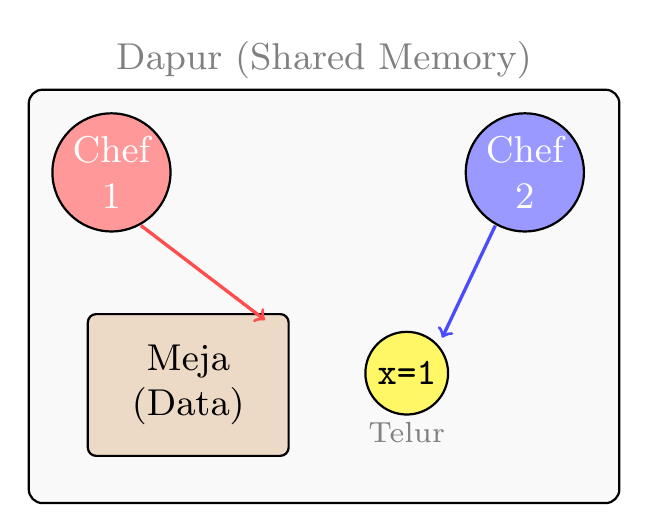
\begin{tikzpicture}[scale=1.5, transform shape]
        % Dapur (kitchen)
        \draw[thick, rounded corners=5pt, fill=gray!5] (0,0) rectangle (5, 3.5);
        \node[font=\small, gray] at (2.5, 3.75) {Dapur (Shared Memory)};

        % Meja
        \draw[fill=brown!30, thick, rounded corners=3pt] (0.5, 0.4) rectangle (2.2, 1.6);
        \node[font=\small, align=center] at (1.35, 1) {Meja\\(Data)};

        % Telur (eggs)
        \draw[fill=yellow!60, thick] (3.2, 1.1) circle (0.35);
        \node[font=\small, align=center] at (3.2, 1.1) {\texttt{x=1}};
        \node[font=\scriptsize, gray] at (3.2, 0.6) {Telur};

        % Chef 1
        \draw[fill=red!40, thick] (0.7, 2.8) circle (0.5);
        \node[font=\small, align=center, text=white] at (0.7, 2.8) {Chef\\1};

        % Chef 2
        \draw[fill=blue!40, thick] (4.2, 2.8) circle (0.5);
        \node[font=\small, align=center, text=white] at (4.2, 2.8) {Chef\\2};

        % Arrows (both reaching for the telur)
        \draw[->, very thick, red!70] (0.95, 2.35) -- (2.0, 1.55);
        \draw[->, very thick, blue!70] (3.95, 2.35) -- (3.5, 1.4);
    \end{tikzpicture}

    \vspace{0.25cm}
    \small\textit{Apa yang terjadi jika keduanya mengambil telur di \textbf{waktu bersamaan}?}
\end{frame}

\begin{frame}
    \frametitle{Analogi: Dua Chef — Pembahasan}
    \framesubtitle{Memetakan analogi ke konsep OS}
    \small

    \begin{columns}[T]
        \column{0.50\textwidth}
        \begin{alertblock}{Skenario Masalah}
            \begin{itemize}
                \item \textbf{Chef 1} ambil telur terakhir
                \item \textbf{Chef 2} juga ambil telur di waktu bersamaan
                \item Hasil: telur hilang — \tem{data rusak!}
            \end{itemize}
        \end{alertblock}

        \column{0.46\textwidth}
        \begin{block}{Analoginya}
            \begin{itemize}
                \item Chef $\rightarrow$ \textbf{thread}
                \item Dapur $\rightarrow$ \textbf{shared memory}
                \item Telur $\rightarrow$ \textbf{shared variable}
            \end{itemize}
        \end{block}
    \end{columns}

    \vspace{0.3cm}
    \begin{exampleblock}{Solusi: Butuh Koordinasi}
        Perlu mekanisme \tem{antrian} atau \tem{zona eksklusif} agar tidak tabrakan — inilah yang akan kita bahas!
    \end{exampleblock}
\end{frame}

\begin{frame}
    \frametitle{Agenda Kelas Hari Ini}
    \framesubtitle{Apa yang kita akan pelajari hari ini}
    \small

    \begin{columns}[T]
        \column{0.48\textwidth}
        \textbf{Bagian 1: Thread Abstraction}

        \vspace{0.1cm}
        Apa itu thread? Bagaimana thread berbeda dari proses? Apa yang \textit{shared} dan apa yang \textit{private}?

        \vspace{0.35cm}
        \textbf{Bagian 2: Race Condition}

        \vspace{0.1cm}
        Apa itu \textit{race condition}? Kenapa \texttt{counter++} bisa menghasilkan nilai salah?

        \column{0.48\textwidth}
        \textbf{Bagian 3: Critical Section}

        \vspace{0.1cm}
        Apa itu \textit{critical section}? Apa tiga syarat solusinya?

        \vspace{0.35cm}
        \textbf{Bagian 4: Ringkasan \& Latihan}

        \vspace{0.1cm}
        Review konsep, latihan soal, dan Q\&A.
    \end{columns}
\end{frame}

\begin{frame}
    \frametitle{Concurrency vs Parallelism}
    \framesubtitle{Dua konsep yang sering tertukar}
    \small

    \begin{columns}[T]
        \column{0.48\textwidth}
        \begin{block}{Concurrency}
            \textbf{Satu CPU, banyak task} bergantian dengan cepat.\\[0.1cm]
            Terasa berjalan bersamaan, tapi sebenarnya \tem{switching cepat}.
        \end{block}

        \vspace{0.2cm}
        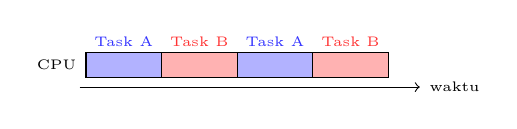
\begin{tikzpicture}[scale=0.8]
            \draw[->] (-0.1, 0) -- (5.3, 0) node[right, font=\tiny]{waktu};
            \draw[fill=blue!30]   (0,   0.15) rectangle (1.2, 0.55);
            \draw[fill=red!30]    (1.2, 0.15) rectangle (2.4, 0.55);
            \draw[fill=blue!30]   (2.4, 0.15) rectangle (3.6, 0.55);
            \draw[fill=red!30]    (3.6, 0.15) rectangle (4.8, 0.55);
            \node[font=\tiny, left] at (0, 0.35) {CPU};
            \node[font=\tiny, blue!80] at (0.6,  0.72) {Task A};
            \node[font=\tiny, red!80]  at (1.8,  0.72) {Task B};
            \node[font=\tiny, blue!80] at (3.0,  0.72) {Task A};
            \node[font=\tiny, red!80]  at (4.2,  0.72) {Task B};
        \end{tikzpicture}

        \vspace{0.1cm}
        \footnotesize\textit{Satu koki bergantian aduk sup dan potong sayur}

        \column{0.48\textwidth}
        \begin{exampleblock}{Parallelism}
            \textbf{Banyak CPU, banyak task} berjalan \tem{benar-benar bersamaan}.
        \end{exampleblock}

        \vspace{0.2cm}
        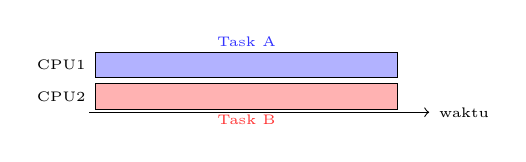
\begin{tikzpicture}[scale=0.8]
            \draw[->] (-0.1, 0) -- (5.3, 0) node[right, font=\tiny]{waktu};
            \draw[fill=blue!30] (0, 0.55) rectangle (4.8, 0.95);
            \draw[fill=red!30]  (0, 0.05) rectangle (4.8, 0.45);
            \node[font=\tiny, left] at (0, 0.75) {CPU1};
            \node[font=\tiny, left] at (0, 0.25) {CPU2};
            \node[font=\tiny, blue!80] at (2.4, 1.12) {Task A};
            \node[font=\tiny, red!80]  at (2.4, -0.12) {Task B};
        \end{tikzpicture}

        \vspace{0.1cm}
        \footnotesize\textit{Dua koki masing-masing mengerjakan tugasnya sendiri}
    \end{columns}
\end{frame}

\begin{frame}
    \frametitle{Checkpoint 0}
    \framesubtitle{Cek pemahaman sebelum lanjut}
    \small

    \begin{enumerate}
        \item Apa perbedaan utama antara \textbf{concurrency} dan \textbf{parallelism}?
        \item Mengapa browser perlu concurrency?
        \item Dalam analogi dapur, apa representasi dari \textit{thread} dan \textit{shared memory}?
    \end{enumerate}

    \vspace{0.3cm}
    \begin{block}{Kunci Jawaban Singkat}
        \small
        \begin{enumerate}
            \item Concurrency = satu CPU switching antar task (ilusi serentak); Parallelism = banyak CPU berjalan benar-benar bersamaan.
            \item Agar download, render, dan input handling bisa terjadi tanpa user freeze.
            \item Chef = thread; Dapur = shared memory; Telur = shared variable.
        \end{enumerate}
    \end{block}
\end{frame}

%================================================
% BAGIAN 1: THREAD ABSTRACTION
%================================================
\section{Thread Abstraction}

\begin{frame}[plain]
    \begin{center}
        \vspace{3cm}
        \Huge\textbf{Thread Abstraction}
    \end{center}
\end{frame}

\begin{frame}
    \frametitle{Thread vs Process}
    \framesubtitle{Perbedaan dan keuntungan thread}
    \footnotesize

    \begin{columns}[T]
        \column{0.50\textwidth}
        \textbf{Masalah dengan Process murni:}
        \begin{itemize}
            \item \textbf{Fork} membuat \tem{copy penuh} address space → mahal
            \item Komunikasi antar proses (IPC) kompleks: pipe, socket
            \item Context switch \textbf{berat}: harus ganti page table
        \end{itemize}

        \vspace{0.2cm}
        \textbf{Thread sebagai solusi:}
        \begin{itemize}
            \item Thread = unit eksekusi \tem{di dalam} proses
            \item Berbagi address space yang sama
            \item Lebih ringan: buat dan switch lebih cepat
        \end{itemize}

        \column{0.46\textwidth}
        \begin{scriptsize}
        \begin{tabular}{p{0.17\textwidth}p{0.27\textwidth}p{0.27\textwidth}}
            \toprule
            \textbf{Aspek} & \textbf{Process} & \textbf{Thread} \\
            \midrule
            Address space & Masing-masing & Shared \\
            Buat overhead & Besar & Kecil \\
            Context switch & Berat & Ringan \\
            Komunikasi & IPC kompleks & Shared mem \\
            Crash satu & Isolasi & Crash proses \\
            \bottomrule
        \end{tabular}
        \end{scriptsize}

        \vspace{0.15cm}
        \begin{alertblock}{Tradeoff}
            \footnotesize Satu thread crash → \tem{seluruh proses} ikut crash.
        \end{alertblock}
    \end{columns}
\end{frame}

\begin{frame}
    \frametitle{Shared vs Private dalam Thread}
    \framesubtitle{Semua thread berbagi satu address space — tapi stack-nya sendiri-sendiri}

    \centering
    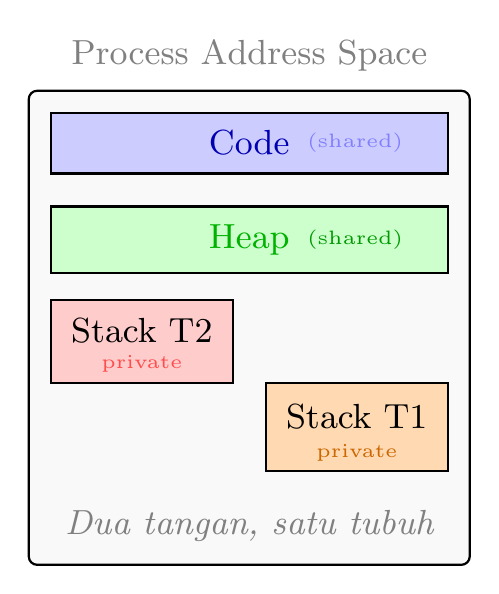
\begin{tikzpicture}[scale=1.4, transform shape]
        \draw[thick, rounded corners=3pt, fill=gray!5] (0, 0) rectangle (4, 4.3);
        \node[font=\small, gray, above] at (2, 4.35) {Process Address Space};

        % Code (shared)
        \draw[fill=blue!20, thick] (0.2, 3.55) rectangle (3.8, 4.1);
        \node[font=\small, text=blue!70!black] at (2, 3.83) {Code};
        \node[font=\tiny, text=blue!50, right] at (2.4, 3.83) {(shared)};

        % Heap (shared)
        \draw[fill=green!20, thick] (0.2, 2.65) rectangle (3.8, 3.25);
        \node[font=\small, text=green!70!black] at (2, 2.95) {Heap};
        \node[font=\tiny, text=green!60!black, right] at (2.4, 2.95) {(shared)};

        % Stack T2 (private)
        \draw[fill=red!20, thick] (0.2, 1.65) rectangle (1.85, 2.4);
        \node[font=\small] at (1.025, 2.13) {Stack T2};
        \node[font=\tiny, text=red!70] at (1.025, 1.82) {private};

        % Stack T1 (private)
        \draw[fill=orange!30, thick] (2.15, 0.85) rectangle (3.8, 1.65);
        \node[font=\small] at (2.975, 1.35) {Stack T1};
        \node[font=\tiny, text=orange!80!black] at (2.975, 1.02) {private};

        % Caption
        \node[font=\small\itshape, align=center, gray] at (2, 0.35) {Dua tangan, satu tubuh};
    \end{tikzpicture}
\end{frame}

\begin{frame}
    \frametitle{Shared vs Private — Detail}
    \framesubtitle{Apa saja yang di-share dan apa yang private?}
    \small

    \begin{columns}[T]
        \column{0.48\textwidth}
        \begin{block}{\textbf{Di-shared} antar thread (1 proses)}
            \begin{itemize}
                \item Code segment
                \item Heap
                \item Global variables
                \item File descriptors
                \item Signal handlers
            \end{itemize}
        \end{block}

        \column{0.48\textwidth}
        \begin{alertblock}{\textbf{Private} per thread}
            \begin{itemize}
                \item Stack (variabel lokal)
                \item Register (termasuk PC)
                \item Thread ID
                \item \texttt{errno}
            \end{itemize}
        \end{alertblock}
    \end{columns}

    \vspace{0.3cm}
    \begin{exampleblock}{Mengapa ini penting?}
        Yang \tem{di-share} bisa menyebabkan konflik jika diakses bersamaan. Yang \tem{private} aman karena hanya dimiliki satu thread.
    \end{exampleblock}
\end{frame}

\begin{frame}
    \frametitle{Thread Control Block \& Thread States}
    \framesubtitle{Tiga keadaan thread dalam sistem operasi}

    \centering
    \vspace{0.3cm}
    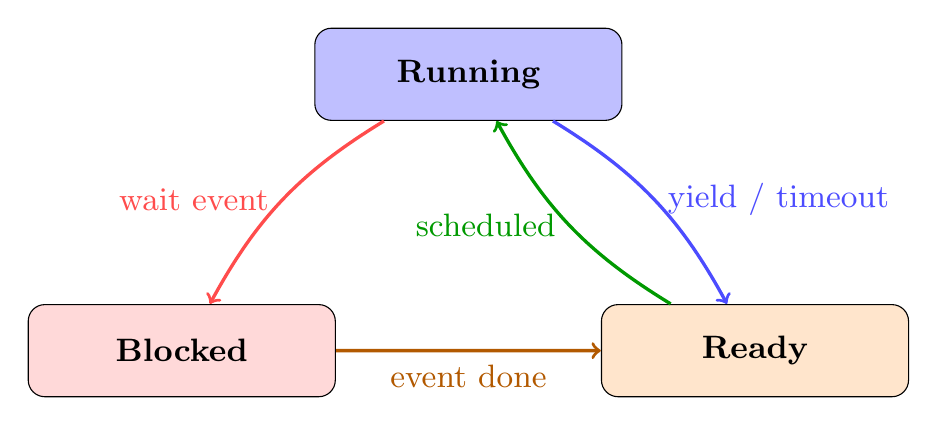
\begin{tikzpicture}[scale=1.3, transform shape,
        state/.style={draw, rounded corners=6pt, minimum width=3cm, minimum height=0.9cm,
                      align=center, font=\small\bfseries},
        arr/.style={->, very thick}
    ]
        \node[state, fill=blue!25] (running) at (3, 3.2) {Running};
        \node[state, fill=orange!20] (ready) at (5.8, 0.5) {Ready};
        \node[state, fill=red!15] (blocked) at (0.2, 0.5) {Blocked};

        \draw[arr, blue!70]        (running) to[bend left=15]  node[right, font=\small]{yield / timeout} (ready);
        \draw[arr, green!60!black]  (ready)   to[bend left=15]  node[left, font=\small]{scheduled} (running);
        \draw[arr, red!70]         (running) to[bend right=15] node[left, font=\small]{wait event} (blocked);
        \draw[arr, orange!70!black] (blocked)  --               node[below, font=\small]{event done} (ready);
    \end{tikzpicture}
\end{frame}

\begin{frame}
    \frametitle{Thread Control Block \& Thread States — Detail}
    \framesubtitle{Bagaimana OS mengelola thread?}
    \small

    \begin{columns}[T]
        \column{0.50\textwidth}
        \textbf{Thread Control Block (TCB):}
        \begin{itemize}
            \item Analogus dengan PCB untuk process
            \item Berisi: register state, stack pointer, PC, thread ID, state
        \end{itemize}

        \vspace{0.2cm}
        \textbf{Thread States:}
        \begin{itemize}
            \item \textbf{Running} — sedang dijalankan CPU
            \item \textbf{Ready} — siap, tapi CPU sedang sibuk
            \item \textbf{Blocked} — menunggu event (I/O, lock)
        \end{itemize}

        \column{0.46\textwidth}
        \begin{block}{Context Switch antar Thread}
            \begin{enumerate}
                \item Simpan register thread lama ke TCB
                \item Muat register thread baru dari TCB
                \item Stack pointer ganti → \tem{stack berbeda}
            \end{enumerate}
        \end{block}
    \end{columns}
\end{frame}

\begin{frame}[fragile]
    \frametitle{Pthread API: Membuat dan Join Thread}
    \framesubtitle{Contoh sederhana dengan pthread}
    \footnotesize

    \begin{columns}[T]
        \column{0.54\textwidth}
        \begin{lstlisting}[basicstyle=\ttfamily\scriptsize, breaklines=true]
#include <stdio.h>
#include <pthread.h>

void *my_thread(void *arg) {
    char *name = (char *) arg;
    printf("Thread %s berjalan\n", name);
    return NULL;
}

int main() {
    pthread_t t1, t2;
    pthread_create(&t1, NULL, my_thread, "A");
    pthread_create(&t2, NULL, my_thread, "B");
    pthread_join(t1, NULL);
    pthread_join(t2, NULL);
    printf("Main selesai\n");
    return 0;
}
        \end{lstlisting}

        \column{0.42\textwidth}
        \begin{block}{Penjelasan Kode}
            \begin{itemize}
                \item \texttt{pthread\_create()}: buat thread baru
                \item \texttt{pthread\_join()}: tunggu thread selesai
            \end{itemize}
        \end{block}

        \vspace{0.2cm}
        \begin{alertblock}{Apakah output selalu berurutan?}
            \texttt{Thread A → Thread B → Main}?

            \vspace{0.1cm}
            \textbf{Tidak!} Urutan bisa berubah — ini disebut \tem{non-determinism}.
        \end{alertblock}
    \end{columns}
\end{frame}

\begin{frame}[fragile]
    \frametitle{Coba Sendiri: Thread Basic}
    \framesubtitle{\texttt{01\_thread\_basic.c} — jalankan dan amati urutannya}
    \small

    \begin{columns}[T]
        \column{0.50\textwidth}
        \begin{block}{Compile \& Jalankan}
            \begin{lstlisting}[basicstyle=\ttfamily\scriptsize]
cd 4_handson_code/week10
make
./01_thread_basic
            \end{lstlisting}
        \end{block}

        \column{0.46\textwidth}
        \begin{exampleblock}{Yang perlu diamati}
            Jalankan \textbf{beberapa kali} — apakah urutan\\\texttt{Thread A} dan \texttt{Thread B} selalu sama?
        \end{exampleblock}

        \vspace{0.15cm}
        \footnotesize Ini membuktikan \tem{non-determinism} pada program concurrent.
    \end{columns}
\end{frame}

\begin{frame}
    \frametitle{Checkpoint 1}
    \framesubtitle{Cek pemahaman Bagian 1}
    \small

    \begin{enumerate}
        \item Sebutkan tiga sumber daya yang di-\textbf{shared} antar thread dalam satu proses.
        \item Sebutkan dua sumber daya yang \textbf{private} per thread.
        \item Pada contoh kode \texttt{pthread\_create}, apakah urutan output \textit{Thread A} dan \textit{Thread B} selalu sama? Mengapa?
        \item Bagaimana OS melakukan \textit{context switch} antar thread?
    \end{enumerate}

    \vspace{0.3cm}
    \begin{block}{Kunci Jawaban Singkat}
        \begin{enumerate}
            \item Shared: code segment, heap, file descriptors
            \item Private: stack, register (termasuk PC)
            \item Tidak — urutan ditentukan scheduler (\textit{non-determinism}).
            \item Simpan register ke TCB lama, muat dari TCB baru, ganti stack pointer.
        \end{enumerate}
    \end{block}
\end{frame}

%================================================
% BAGIAN 2: RACE CONDITION
%================================================
\section{Race Condition}

\begin{frame}[plain]
    \begin{center}
        \vspace{3cm}
        \Huge\textbf{Race Condition}
    \end{center}
\end{frame}

\begin{frame}[fragile]
    \frametitle{Kode yang Tampak Benar}
    \framesubtitle{Dua thread, satu counter shared}
    \scriptsize

    \begin{columns}[T]
        \column{0.58\textwidth}
        \begin{lstlisting}[basicstyle=\ttfamily\scriptsize, breaklines=true]
#include <stdio.h>
#include <pthread.h>

int counter = 0;   // shared!

void *increment(void *arg) {
    for (int i = 0; i < 1000000; i++) {
        counter++;
    }
    return NULL;
}

int main() {
    pthread_t t1, t2;
    pthread_create(&t1, NULL, increment, NULL);
    pthread_create(&t2, NULL, increment, NULL);
    pthread_join(t1, NULL);
    pthread_join(t2, NULL);
    printf("counter = %d\n", counter);
    return 0;
}
        \end{lstlisting}

        \column{0.38\textwidth}
        \begin{block}{Prediksi Awal}
            \small Dua thread masing-masing melakukan 1.000.000 increment.

            \vspace{0.15cm}
            \centering
            \Large\texttt{counter = 2000000}
        \end{block}

        \vspace{0.2cm}
        \begin{alertblock}{Pertanyaan}
            Apakah hasilnya \textbf{selalu} 2.000.000?
        \end{alertblock}
    \end{columns}
\end{frame}

\begin{frame}[fragile]
    \frametitle{Coba Sendiri: Race Condition}
    \framesubtitle{\texttt{02\_race\_condition.c} — lihat race condition langsung}
    \small

    \begin{columns}[T]
        \column{0.50\textwidth}
        \begin{block}{Compile \& Jalankan}
            \begin{lstlisting}[basicstyle=\ttfamily\scriptsize]
gcc -Wall -pthread -O0 \
  -o 02_race 02_race_condition.c
./02_race
            \end{lstlisting}
        \end{block}

        \column{0.46\textwidth}
        \begin{alertblock}{Yang perlu diamati}
            Jalankan \textbf{3--5 kali}. Apakah hasilnya selalu 2.000.000? Berapa banyak update yang hilang?
        \end{alertblock}
    \end{columns}
\end{frame}

\begin{frame}
    \frametitle{Hasil Nyata: Tidak Stabil}
    \framesubtitle{Program yang sama, output bisa berbeda}
    \small

    \begin{columns}[T]
        \column{0.48\textwidth}
        \begin{block}{Ekspektasi}
            \centering
            \Large\texttt{2000000}
        \end{block}

        \vspace{0.2cm}
        \begin{exampleblock}{Bayangkan...}
            Dua kasir menghitung stok barang di papan yang sama. Keduanya berniat benar, tapi kalau tulis-hapusnya bertabrakan, angka akhir bisa salah.
        \end{exampleblock}

        \column{0.48\textwidth}
        \begin{alertblock}{Beberapa hasil run}
            \begin{itemize}
                \item \texttt{counter = 1234512}
                \item \texttt{counter = 1876023}
                \item \texttt{counter = 1543781}
            \end{itemize}
        \end{alertblock}

        \vspace{0.15cm}
        \centering
        \Large\tem{Tidak selalu 2.000.000!}
    \end{columns}
\end{frame}

\begin{frame}[fragile]
    \frametitle{\texttt{counter++} Bukan Satu Instruksi}
    \framesubtitle{Satu baris C bisa pecah jadi beberapa langkah mesin}
    \scriptsize

    \begin{columns}[T]
        \column{0.30\textwidth}
        \begin{block}{Di kode C}
            \centering
            \Huge\texttt{counter++}
        \end{block}

        \vspace{0.2cm}
        \begin{exampleblock}{Pesan utama}
            \small Satu baris C terlihat sederhana, tapi CPU melihatnya sebagai \tem{tiga langkah terpisah}.
        \end{exampleblock}

        \column{0.66\textwidth}
        \begin{block}{Di level assembly}
\begin{lstlisting}[basicstyle=\ttfamily\scriptsize]
MOV eax, [counter]   ; LOAD  nilai dari memori
ADD eax, 1           ; ADD   tambah 1 di register
MOV [counter], eax   ; STORE tulis balik ke memori
\end{lstlisting}
        \end{block}

        \vspace{0.1cm}
        \scriptsize
        \begin{tabular}{p{0.16\textwidth}p{0.46\textwidth}}
            \toprule
            \textbf{Langkah} & \textbf{Makna} \\
            \midrule
            LOAD & Baca nilai lama ke register \\
            ADD & Tambah 1 di register \\
            STORE & Tulis hasil ke memori \\
            \bottomrule
        \end{tabular}
    \end{columns}
\end{frame}

\begin{frame}
    \frametitle{Interleaving yang Bermasalah}
    \framesubtitle{Masalah muncul saat dua thread saling menyela}
    \footnotesize

    \begin{block}{Setup}
        Nilai awal \texttt{counter = 50}. Dua thread sama-sama menjalankan \texttt{counter++}.
    \end{block}

    \vspace{0.15cm}
    \begin{columns}[T]
        \column{0.48\textwidth}
        \begin{block}{Urutan kejadian}
            \begin{enumerate}
                \item T1: LOAD $\rightarrow$ register = 50
                \item OS \textit{preempt} T1
                \item T2: LOAD, ADD, STORE $\rightarrow$ \texttt{counter = 51}
                \item T1 lanjut: ADD, STORE $\rightarrow$ tetap 51
            \end{enumerate}
        \end{block}

        \column{0.48\textwidth}
        \begin{block}{Evolusi nilai}
            \scriptsize
            \begin{tabular}{p{0.22\textwidth}p{0.14\textwidth}}
                \toprule
                \textbf{Momen} & \textbf{Nilai} \\
                \midrule
                Awal & 50 \\
                T1 selesai LOAD & 50 \\
                T2 selesai STORE & 51 \\
                T1 selesai STORE & 51 \\
                \bottomrule
            \end{tabular}

            \vspace{0.1cm}
            \textbf{Inti:} dua thread sama-sama membaca 50.
        \end{block}
    \end{columns}
\end{frame}

\begin{frame}
    \frametitle{Lost Update}
    \framesubtitle{Hasil akhir salah walau tiap thread tampak benar}
    \small

    \begin{columns}[T]
        \column{0.46\textwidth}
        \begin{alertblock}{Seharusnya}
            \centering
            \Large 50 + 1 + 1 = \textbf{52}
        \end{alertblock}

        \vspace{0.2cm}
        \begin{block}{Yang benar-benar terjadi}
            \centering
            \Large hasil akhir = \textbf{51}
        \end{block}

        \column{0.50\textwidth}
        \begin{exampleblock}{Analogi papan tulis}
            Bayangkan dua orang melihat angka 50 di papan tulis, lalu keduanya menghitung ``50 + 1'' di kepala masing-masing. Saat menulis balik, keduanya sama-sama menulis 51. Satu update hilang.
        \end{exampleblock}

        \vspace{0.15cm}
        \centering
        \Large\tem{Inilah lost update.}
    \end{columns}
\end{frame}

\begin{frame}
    \frametitle{Kapan Aman, Kapan Bahaya?}
    \framesubtitle{Tidak semua akses bersamaan otomatis salah}
    \small

    \begin{columns}[T]
        \column{0.48\textwidth}
        \begin{exampleblock}{Aman}
            \begin{itemize}
                \item Tiap thread bekerja pada \textbf{data private}
                \item Variabel lokal ada di \textbf{stack masing-masing}
                \item Thread tidak saling menimpa hasil
            \end{itemize}
        \end{exampleblock}

        \column{0.48\textwidth}
        \begin{alertblock}{Bahaya}
            \begin{itemize}
                \item Banyak thread menyentuh \textbf{data shared}
                \item Update terjadi hampir bersamaan
                \item Urutan eksekusi berubah-ubah
            \end{itemize}
        \end{alertblock}
    \end{columns}

    \vspace{0.2cm}
    \begin{block}{Aturan cepat}
        Kalau pertanyaannya menyangkut \tem{siapa yang boleh menyentuh data yang sama pada waktu yang sama}, kita mulai masuk wilayah \textit{race condition}.
    \end{block}
\end{frame}

\begin{frame}
    \frametitle{Analogi Sederhana: Dua Kasir, Satu Catatan Stok}
    \framesubtitle{Mengapa hasil bisa salah padahal semua orang berniat benar?}
    \small

    \begin{columns}[T]
        \column{0.52\textwidth}
        \begin{block}{Skenario}
            \begin{enumerate}
                \item Stok awal tertulis \textbf{50}
                \item Kasir A membaca angka itu
                \item Sebelum A menulis balik, Kasir B juga membaca \textbf{50}
                \item Keduanya menulis hasil ``51''
            \end{enumerate}
        \end{block}

        \column{0.44\textwidth}
        \begin{exampleblock}{Pelajarannya}
            Masalahnya bukan karena salah hitung.

            \vspace{0.15cm}
            Masalahnya karena \tem{dua orang memakai catatan yang sama tanpa koordinasi}.
        \end{exampleblock}
    \end{columns}

    \vspace{0.2cm}
    \begin{alertblock}{Hubungan ke thread}
        Kasir = thread, catatan stok = shared variable, tulis balik = STORE ke memori.
    \end{alertblock}
\end{frame}

\begin{frame}
    \frametitle{Definisi Race Condition}
    \framesubtitle{Kapan kita bilang sebuah program terkena race condition?}
    \small

    \begin{block}{Definisi}
        \textit{Race condition} adalah kondisi ketika hasil eksekusi program bergantung pada \tem{timing} atau \tem{urutan} eksekusi dua atau lebih thread yang mengakses data yang sama.
    \end{block}

    \vspace{0.2cm}
    \begin{columns}[T]
        \column{0.48\textwidth}
        \begin{itemize}
            \item \textbf{Non-deterministic}: kadang benar, kadang salah
            \item Sulit di-debug karena tidak selalu muncul
        \end{itemize}

        \column{0.48\textwidth}
        \begin{itemize}
            \item Bergantung pada scheduler dan timing CPU
            \item Makin berbahaya saat beban sistem tinggi
        \end{itemize}
    \end{columns}
\end{frame}

\begin{frame}[fragile]
    \frametitle{Latihan: Race Condition atau Tidak?}
    \framesubtitle{Kuncinya: shared atau private?}
    \scriptsize

    \begin{columns}[T]
        \column{0.48\textwidth}
        \begin{block}{Soal 1}
\begin{lstlisting}[basicstyle=\ttfamily\scriptsize, breaklines=true]
void transfer(int amount) {
    balance_A -= amount;
    balance_B += amount;
}
\end{lstlisting}
        \end{block}

        \begin{alertblock}{Jawaban}
            \textbf{Ya, bisa race condition.} \texttt{balance\_A} dan \texttt{balance\_B} adalah shared data.
        \end{alertblock}

        \column{0.48\textwidth}
        \begin{block}{Soal 2}
\begin{lstlisting}[basicstyle=\ttfamily\scriptsize, breaklines=true]
void calculate(int x) {
    int local = x * 2;
    printf("%d\n", local);
}
\end{lstlisting}
        \end{block}

        \begin{exampleblock}{Jawaban}
            \textbf{Tidak, jika \texttt{local} benar-benar variabel lokal.} Ia berada di stack private milik tiap thread.
        \end{exampleblock}
    \end{columns}
\end{frame}

\begin{frame}
    \frametitle{Checkpoint 2}
    \framesubtitle{Cek pemahaman Bagian 2}
    \small

    \begin{enumerate}
        \item Mengapa \texttt{counter++} tidak aman jika dua thread mengakses \texttt{counter} yang sama?
        \item Dalam contoh \textit{interleaving}, mengapa hasil akhir bisa 51 padahal seharusnya 52?
        \item Apa arti \textit{non-determinism} pada program concurrent?
    \end{enumerate}

    \vspace{0.3cm}
    \begin{block}{Kunci Jawaban Singkat}
        \begin{enumerate}
            \item Karena \texttt{counter++} terdiri dari LOAD, ADD, dan STORE yang bisa disela thread lain.
            \item Kedua thread membaca nilai lama yang sama, lalu salah satu update menimpa update lainnya.
            \item Program yang sama bisa memberi hasil atau urutan berbeda karena timing eksekusi tidak tetap.
        \end{enumerate}
    \end{block}
\end{frame}

%================================================
% BAGIAN 3: CRITICAL SECTION
%================================================
\section{Critical Section}

\begin{frame}[plain]
    \begin{center}
        \vspace{3cm}
        \Huge\textbf{Critical Section}
    \end{center}
\end{frame}

\begin{frame}[fragile]
    \frametitle{Apa Itu Critical Section?}
    \framesubtitle{Bagian kode yang tidak boleh dipakai bersamaan}
    \small

    \begin{block}{Definisi}
        \textit{Critical section} adalah bagian kode yang mengakses \tem{shared resource} dan tidak boleh dieksekusi oleh lebih dari satu thread pada saat yang sama.
    \end{block}

    \vspace{0.2cm}
    \begin{columns}[T]
        \column{0.48\textwidth}
        \begin{alertblock}{Contoh critical section}
\begin{lstlisting}[basicstyle=\ttfamily\scriptsize]
counter++;   // shared variable
\end{lstlisting}
            Di sini dua thread bisa menabrak data yang sama.
        \end{alertblock}

        \column{0.48\textwidth}
        \begin{exampleblock}{Bukan critical section}
\begin{lstlisting}[basicstyle=\ttfamily\scriptsize]
int temp = x * 2;
printf("%d\n", temp);
\end{lstlisting}
            \texttt{temp} adalah variabel lokal di stack private.
        \end{exampleblock}
    \end{columns}
\end{frame}

\begin{frame}
    \frametitle{Visualisasi Critical Section}
    \framesubtitle{Yang tidak boleh overlap adalah bagian kritisnya}
    \small

    \begin{center}
    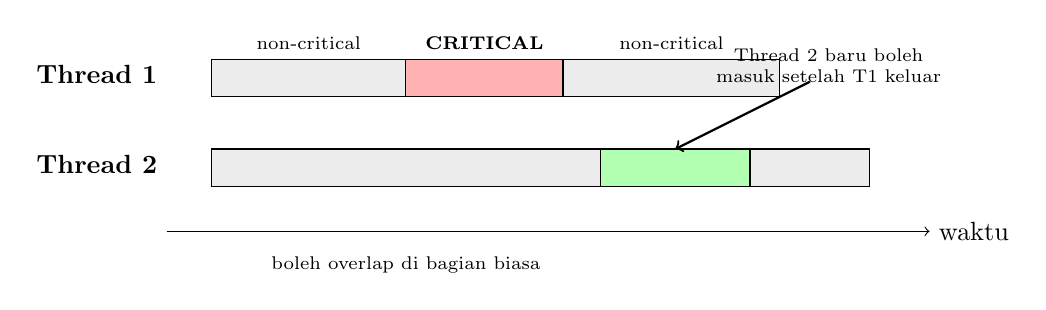
\begin{tikzpicture}[scale=0.95, transform shape]
        \draw[->] (0,0) -- (10.2,0) node[right]{waktu};

        \node[left] at (0,2.1) {\textbf{Thread 1}};
        \draw[fill=gray!15] (0.6,1.8) rectangle (3.2,2.3);
        \draw[fill=red!30]  (3.2,1.8) rectangle (5.3,2.3);
        \draw[fill=gray!15] (5.3,1.8) rectangle (8.2,2.3);

        \node[left] at (0,0.9) {\textbf{Thread 2}};
        \draw[fill=gray!15] (0.6,0.6) rectangle (5.8,1.1);
        \draw[fill=green!30] (5.8,0.6) rectangle (7.8,1.1);
        \draw[fill=gray!15] (7.8,0.6) rectangle (9.4,1.1);

        \node[font=\scriptsize] at (1.9,2.52) {non-critical};
        \node[font=\scriptsize] at (4.25,2.52) {\textbf{CRITICAL}};
        \node[font=\scriptsize] at (6.75,2.52) {non-critical};

        \node[font=\scriptsize] at (3.2,-0.45) {boleh overlap di bagian biasa};
        \draw[->, thick] (8.6,2.0) -- (6.8,1.1);
        \node[font=\scriptsize, align=center] at (8.85,2.22) {Thread 2 baru boleh\\masuk setelah T1 keluar};
    \end{tikzpicture}
    \end{center}

    \vspace{0.2cm}
    \begin{exampleblock}{Analogi}
        Bayangkan hanya ada \tem{satu kunci} untuk ruang arsip. Siapa pun yang sedang di dalam, orang lain harus menunggu di luar.
    \end{exampleblock}
\end{frame}

\begin{frame}
    \frametitle{Tiga Syarat Solusi Critical Section}
    \framesubtitle{Solusi yang benar tidak cukup hanya ``mengunci''}
    \small

    \begin{columns}[T]
        \column{0.32\textwidth}
        \begin{block}{1. Mutual Exclusion}
            Hanya \textbf{satu thread} yang boleh ada di critical section pada satu waktu.
        \end{block}

        \column{0.32\textwidth}
        \begin{exampleblock}{2. Progress}
            Kalau critical section kosong dan ada yang ingin masuk, harus ada keputusan masuk dalam waktu terbatas.
        \end{exampleblock}

        \column{0.32\textwidth}
        \begin{alertblock}{3. Bounded Waiting}
            Thread yang sudah meminta masuk tidak boleh menunggu tanpa batas.
        \end{alertblock}
    \end{columns}
\end{frame}

\begin{frame}
    \frametitle{Kalau Syaratnya Dilanggar, Apa yang Terjadi?}
    \framesubtitle{Tiap syarat mencegah masalah yang berbeda}
    \scriptsize

    \begin{tabular}{p{0.21\textwidth}p{0.29\textwidth}p{0.33\textwidth}}
        \toprule
        \textbf{Syarat} & \textbf{Pertanyaan kunci} & \textbf{Jika gagal} \\
        \midrule
        Mutual Exclusion & Apakah maksimum satu thread ada di CS? & \textit{Race condition} tetap terjadi \\
        Progress & Jika CS kosong, apakah ada yang bisa segera masuk? & Bisa macet atau saling tunggu \\
        Bounded Waiting & Apakah ada batas menunggu? & Satu thread bisa kelaparan (\textit{starvation}) \\
        \bottomrule
    \end{tabular}

    \vspace{0.25cm}
    \begin{block}{Cara mudah mengingat}
        \textbf{ME} mencegah tabrakan, \textbf{Progress} mencegah mandek, \textbf{Bounded Waiting} mencegah dianaktirikan.
    \end{block}
\end{frame}

\begin{frame}[fragile]
    \frametitle{Percobaan Naif 1: Flag Sederhana}
    \framesubtitle{Kelihatannya masuk akal, tapi bisa macet}
    \scriptsize

    \begin{columns}[T]
        \column{0.54\textwidth}
\begin{lstlisting}[basicstyle=\ttfamily\scriptsize, breaklines=true]
int flag[2] = {0, 0};

// Thread 0
flag[0] = 1;
while (flag[1]);
// critical section
flag[0] = 0;
\end{lstlisting}

        \column{0.42\textwidth}
        \begin{alertblock}{Masalah}
            Jika Thread 0 dan Thread 1 sama-sama set flag menjadi 1 hampir bersamaan, keduanya akan saling menunggu.
        \end{alertblock}

        \begin{block}{Akibat}
            Tidak ada yang maju. Ini melanggar \tem{progress}.
        \end{block}
    \end{columns}
\end{frame}

\begin{frame}[fragile]
    \frametitle{Percobaan Naif 2: Turn Variable}
    \framesubtitle{Tidak tabrakan, tapi terlalu kaku}
    \scriptsize

    \begin{columns}[T]
        \column{0.54\textwidth}
\begin{lstlisting}[basicstyle=\ttfamily\scriptsize, breaklines=true]
int turn = 0;

// Thread 0
while (turn != 0);
// critical section
turn = 1;
\end{lstlisting}

        \column{0.42\textwidth}
        \begin{alertblock}{Masalah}
            Thread 1 tidak bisa masuk dua kali berturut-turut kalau Thread 0 belum ``memberi giliran'', meski CS sedang kosong.
        \end{alertblock}

        \begin{block}{Akibat}
            Solusi ini juga gagal memenuhi \tem{progress}.
        \end{block}
    \end{columns}
\end{frame}

\begin{frame}
    \frametitle{Jadi, Kita Butuh Apa?}
    \framesubtitle{Teaser ke pertemuan berikutnya}
    \small

    \begin{block}{Kesimpulan section ini}
        Kita butuh mekanisme yang:
        \begin{itemize}
            \item mencegah dua thread masuk bersamaan,
            \item tidak membuat semua thread macet,
            \item dan tetap adil untuk yang menunggu.
        \end{itemize}
    \end{block}

    \vspace{0.2cm}
    \begin{exampleblock}{Preview minggu berikutnya}
        Di sinilah \tem{lock} dan \tem{mutex} masuk. Kita akan belajar bagaimana hardware dan OS membantu membuat critical section benar-benar aman.
    \end{exampleblock}
\end{frame}

\begin{frame}[fragile]
    \frametitle{Coba Sendiri: Mutex vs Flag Naif}
    \framesubtitle{\texttt{03\_mutex\_fix.c} \& \texttt{04\_naive\_flag.c} — bandingkan keduanya}
    \small

    \begin{columns}[T]
        \column{0.48\textwidth}
        \begin{exampleblock}{03: Mutex yang benar}
            \begin{lstlisting}[basicstyle=\ttfamily\scriptsize]
./03_mutex_fix
# Selalu: Hasil nyata: 2000000
            \end{lstlisting}
            Mutual exclusion terpenuhi — hasilnya \textbf{selalu} tepat.
        \end{exampleblock}

        \column{0.48\textwidth}
        \begin{alertblock}{04: Flag naif (bisa hang!)}
            \begin{lstlisting}[basicstyle=\ttfamily\scriptsize]
./04_naive_flag
# Mungkin tidak selesai
# Ctrl+C untuk keluar
            \end{lstlisting}
            Syarat \tem{progress} dilanggar — bisa \textit{deadlock}.
        \end{alertblock}
    \end{columns}
\end{frame}

\begin{frame}
    \frametitle{Checkpoint 3}
    \framesubtitle{Cek pemahaman Bagian 3}
    \scriptsize

    \begin{enumerate}
        \item Apa yang dimaksud dengan \textit{critical section}?
        \item Mengapa \texttt{counter++} termasuk critical section?
        \item Apa beda \textit{mutual exclusion}, \textit{progress}, dan \textit{bounded waiting}?
        \item Mengapa solusi flag sederhana bisa membuat sistem macet?
    \end{enumerate}

    \vspace{0.3cm}
    \begin{block}{Kunci Jawaban Singkat}
        \begin{enumerate}
            \item Bagian kode yang mengakses data shared dan tidak boleh dieksekusi bersamaan.
            \item Karena ia menyentuh variabel shared.
            \item ME: cegah tabrakan; progress: cegah mandek; bounded waiting: cegah starvation.
            \item Karena dua thread bisa saling menunggu.
        \end{enumerate}
    \end{block}
\end{frame}

%================================================
% BAGIAN 4: RINGKASAN & PENUTUP
%================================================
\section{Ringkasan \& Penutup}

\begin{frame}[plain]
    \begin{center}
        \vspace{3cm}
        \Huge\textbf{Ringkasan \& Penutup}
    \end{center}
\end{frame}

\begin{frame}
    \frametitle{Rangkuman: Tiga Ide Besar Hari Ini}
    \framesubtitle{Kalau pulang hanya bawa tiga hal, bawa tiga ini}
    \scriptsize

    \begin{tabular}{p{0.22\textwidth}p{0.24\textwidth}p{0.39\textwidth}}
        \toprule
        \textbf{Topik} & \textbf{Kata kunci} & \textbf{Inti} \\
        \midrule
        Thread & shared vs private & Banyak jalur eksekusi dalam satu proses, berbagi address space yang sama \\
        Race Condition & timing matters & Hasil program bisa berubah karena urutan eksekusi thread tidak tetap \\
        Critical Section & perlu proteksi & Bagian yang menyentuh data shared harus dijaga agar tidak dipakai bersamaan \\
        \bottomrule
    \end{tabular}

    \vspace{0.25cm}
    \begin{exampleblock}{Kalimat paling singkat}
        \tem{Thread membuat program lebih responsif}, tapi \tem{shared data} membuat kita harus hati-hati.
    \end{exampleblock}
\end{frame}

\begin{frame}
    \frametitle{Checklist Keterampilan}
    \framesubtitle{Coba cek, mana yang sudah terasa paham?}
    \small

    \begin{columns}[T]
        \column{0.48\textwidth}
        \begin{itemize}
            \item Menjelaskan beda \textit{thread} dan \textit{process}
            \item Menyebutkan mana yang \textit{shared} dan mana yang private
            \item Membaca contoh kode \texttt{pthread}
            \item Menjelaskan kenapa \texttt{counter++} bisa salah
        \end{itemize}

        \column{0.48\textwidth}
        \begin{itemize}
            \item Menggambar interleaving yang memicu \textit{lost update}
            \item Mendefinisikan \textit{race condition}
            \item Menjelaskan \textit{critical section}
            \item Menyebutkan tiga syarat solusi yang benar
        \end{itemize}
    \end{columns}
\end{frame}

\begin{frame}
    \frametitle{Kuis Penutup}
    \framesubtitle{Cek cepat sebelum kita akhiri}
    \small

    \begin{enumerate}
        \item Sebutkan 3 hal yang di-\textit{share} dan 2 hal yang private per thread.
        \item Jika dua thread masing-masing menjalankan \texttt{x = x + 1} pada variabel global \texttt{x} yang awalnya 0, nilai akhir \texttt{x} bisa berapa?
        \item Jika hanya satu thread boleh masuk critical section, tetapi thread lain bisa menunggu selamanya, syarat mana yang dilanggar?
    \end{enumerate}

    \vspace{0.3cm}
    \begin{block}{Kunci singkat}
        Shared: code, heap, global variable. Private: stack, register. Nilai akhir \texttt{x} bisa 1 atau 2. Jika ada yang menunggu selamanya, yang gagal adalah \textit{bounded waiting}.
    \end{block}
\end{frame}

\begin{frame}
    \frametitle{Terima Kasih}
    \begin{center}
        \Huge \textbf{Ada Pertanyaan?}

        \vspace{0.8cm}
        \normalsize
        Minggu depan kita masuk ke cara nyata melindungi \textit{critical section} dengan \tem{lock} dan \tem{mutex}.

        \vspace{0.8cm}
        \small
        \textit{``Programs must be written for people to read, and only incidentally for machines to execute.''} \\
        \vspace{0.1cm}
        --- Harold Abelson
    \end{center}
\end{frame}

\end{document}
